\chapter{Lyrics-based methods}
 In this chapter we will briefly describe some of the most prominent methods to represent songs based on their lyrics. After specifically focusing on the positive and negative aspects of these methods, we will select suitable candidates for testing and our web application.
\section{Related work}

The reason to explore lyrics-based methods in this thesis is based on several factors. First of all I believe that although it is not a completely unexplored area, there are several papers and on this topic \cite{Gossi2016LyricBasedMR}, \cite{DBLP:journals/corr/Tsaptsinos17}, \cite{inproceedings} I have not found any recommendation system or application that would recommend songs solely based on their lyrics and I am curious about the results, so admittedly, this is of my personal curiosity. Secondly I also believe that the main advantage of these methods could be the variety of recommendations, that still will not be completely off as for example a simple TF-IDF song embedding proved to be 12.6 times more accurate then just random suggestions \cite{Gossi2016LyricBasedMR}.

\section{Text embedding methods}
\subsection{Bag of Words}
The Bag of Words commonly referred to as BoW is a text representation which counts how many times a word appears in a document, in my \todo[inline]{LP: spis neco jako "in the context of this thesis a word appears in the song lyrics"} case it would be how many times a word comes up in a song.
Every song would be represented as a wordcount vector where each index corresponds to the number times a certain word appeared in the song. \todo[inline]{LP: Mozna pridat info o tom, ze BOW je zakladni reprezentace a trpi nejakymi problemy (stopwords, ruzne dlouhe texty), ktere se TF-IDF snazi resit}
\subsection{TF-IDF}
Term Frequency-Inverse Document Frequency is another way to represent documents in a more mathematically friendly way. Unlike the BoW, TF-IDF does not measure the frequency of words in a document but it measures the relevance them \todo[inline]{LP: their relevance}. As can be deduced from the title term frequency, first the number of appearances of a word in each document - \textit{tf} - \todo[inline]{LP: pozor, term frequency neni pocet, ale pomer (tj, pokud z 10 slov je 3x slovo já, tak bude mit tf=0.3 a ne 3 - to je ochrana proti ruzne dlouhym dokumentum}is computed but then comes the inverse document frequency part - \textit{idf} - where the words are weighted as seen in (3.1). The words that appear frequently in all documents have lower weights and those who only appear in some have higher weights.

\begin{equation}
idf(t) = log\frac{1+n_d}{1+df(d,t)} + 1
\end{equation}

\begin{equation}
tf\textnormal{-}idf(t,d) = idf(t)*tf(t,d) 
\end{equation}

where \textit{t} is the word and \textit{d} is the document and \textit{n\textsubscript{d}} is the total number of documents.\todo[inline]{LP: trochu mi ta rovnice 3.1 nesedi - ve jmenovateli ma byt pocet dokumentu s vyskytem slova t a na to mi $df(d,t)$ moc nesedi - jeste na to mrknete.} 

\subsection{Word2Vec}
Word2Vec is a two-layer neural network trained to encode a linguistic context of a word. Each word has a vector assigned in a vector space of typically hundreds of dimensions) generated from a large corpus. The position of a word corresponds to its context, meaning, that words that share common context are closer to each other. \\
There are two possible Word2Vec architectures, the continuous bag-of-words or a continuous skip gram. The CBOW predicts the current word from the words surrounding it which is the context. It does not keep the order of the surrounding context words.The skip gram does, which makes it slower but also more effective, especially for infrequent words \cite{DBLP:journals/corr/abs-1301-3781}. The Skip-Gram architecture takes one word and predicts all the context around it.
\begin{figure}[h]
    \centering
	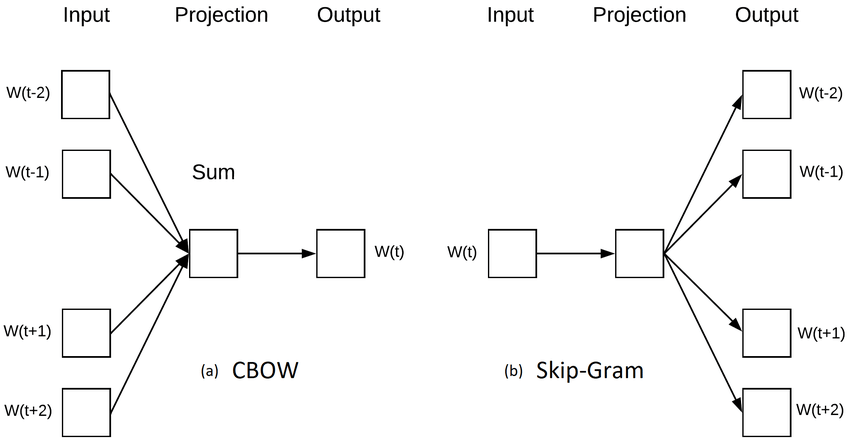
\includegraphics[height=70mm]{./img/cbow_skipgram_w2v_architecture.png}
	\caption{The CBOW and Skip-gram Word2Vec architectures}
	\label{fig:cbow_skipgram_w2v_architecture}
\end{figure}
\\
\todo[inline]{LP: pokud je ten obrazek prevzaty, nezapomen doplnit zdroj (pokud jsi ho kreslila sama, OK (ono neni tak tezke to nakreslit, tak pokud jste to neudelala, udelejte:-))}
Multiple things have to be taken into account when training a W2V model. The information value of words that occur in all training document is quite low so they can be removed to increase training speed. The dimensionality of the space also brings up accuracy only to a certain point so some threshold has to be set. Another parameter is the context window, which determines, how many word before and after a given word are included as its context.

\subsection{Doc2Vec}
Doc2Vec as is an unsupervised algorithm that learns the feature representation of texts with various lengths and encodes them into vectors of the same length. As the name suggests it is heavily based on the idea of Word2Vec. It was also first presented by the same group of researches in this paper \cite{DBLP:journals/corr/LeM14}. The main idea of the method is to use the word2vec model but add one more vector to represent the paragraph as a whole. As in the Word2Vec model, there are two architectures for the Doc2Vec approach. The Distributed Memory (DM) version of Paragraph vector and the Distributed Bag of Words (DBOW) version of the Paragraph vector. Again, the DBOW is faster but does not consider the order of the words as it predicts a random group of words from just the paragraph vector. The DM on the other hand takes previous words and the paragraph vector into account and predicts just one word. This way, because the paragraph does not shift across the text, the DM architecture is able to capture some word order.
\begin{figure}[h]
    \centering
	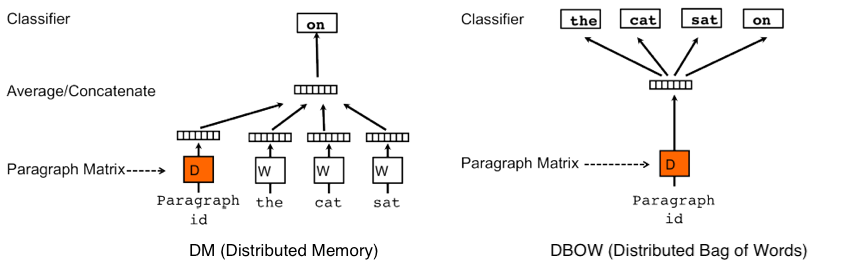
\includegraphics[width=140mm]{./img/DV_DBOW_doc2vec_architectures.png}
	\caption{The Doc2Vec DM and DBOW architecture}
	\label{fig:dbow_dm_d2v_architecture}
\end{figure}
\subsection{Self organizing maps}
Self organizing maps (SOM) is a type of a neural network that learns how to reduce the dimension of input data in an unsupervised manner. SOMs were introduced by Teuvo Kohonen \cite{Kohonen1982}. They use competitive dimensionality reduction (meaning the nodes in the SOM network compete to get the right to respond to the input data) which is quite unusual for neural networks as they usually use backpropagation. The models that SOMs compute is a (usually) two dimensional space of neurons (called \textit{codebook} vectors) where similar examples are close end up to each other and dissimilar examples further from each other.\\
The SOM network is trained through an iterative process. It chooses one sample \textbf{x} \in  $ R^n $ from the input training set at random and teaches it to itself. During teaching, the network feeds the chosen sample into all its' units. A winner unit is calculated based on a similarity measure (usually Euclidean distance) between \textbf{x} and the \textit{codebook} vectors. Finally the values of the network units are updated. The best-matching unit is moved a closer to the \textbf{x} vector and so are all the topological neighbours of the best unit.\\
The neighbours are defined by a neighbourhood function. It decreases with time and decides how radical the change around the winner will be. There are multiple functions that can be used. One can use the Gaussian kernel around the winner, however this is quite computationally expensive. A good and more efficient function is sometimes called the \textit{"bubble"} function which is constant over the whole neighbourhood of the winner and zero elsewhere \cite{SOM_training}.
\begin{figure}[h]
    \centering
	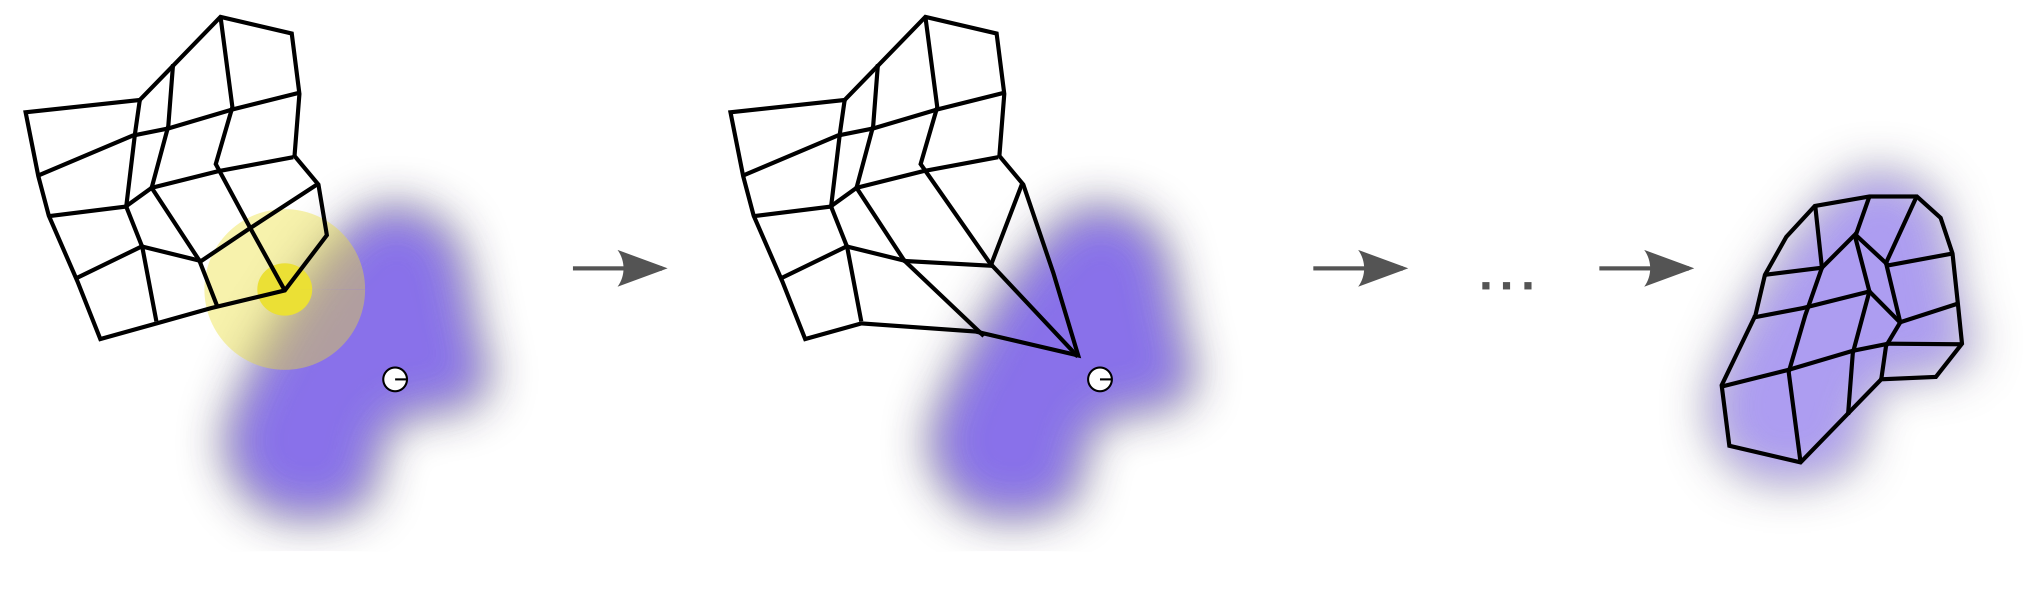
\includegraphics[width=140mm]{./img/Somtraining.png}
	\caption{Visualization of the training algorithm used for SOM networks. The blue area represents the distribution of the data. The white dot is the randomly selected sample. On the left, the SOM network nodes (units) are randomly spread accross the space. When finding a winner (middle) and its defined neighbourhood (the yellow area) the network moves towards the datapoint and eventually after repeated iterations spreads mimicking the distribution of the data (left).}
	\label{fig:som_training}
\end{figure}

\section{Choices for implementation}
When choosing methods for our web application there are several factors to consider. Besides the expected accuracy of the algorithms, which however is often difficult to guess as their abilities to recommend songs based on lyrics have not been researched extensively, we have to consider the implementation as well as speed \todo{LP:temporal complexity nebo time complexity} features of all the methods. Also, the fact that we want to focus more on a cross-sectional approach rather than a thorough optimization of one particular algorithm, means we will prefer diversity in our chosen algorithms. 
\subsection{Text representation choices}
The Bag of Words representation could be a good choice for some kind of baseline results. Nevertheless, since the TF-idf algorithm is widely based on the BOW and is still quite simple, we choose \textbf{TF-idf} as our base. As mentioned at the beginning of this chapter, it was proven to be 12.6 times more accurate than just random suggestions, and that is what we hope to achieve with all of our text methods. A downside of the TF-idf method is the length of its vectors. Even though they consist mostly of zeros, for our dataset, the length of each of them is over 22 000. \todo{LPvyzkouset TF-IDF s redukci na treba 1000 nejcastejsich slov, nebo nejake clusterovani slov. Treba to i zlepsi vysledky...}\\

Word2Vec and Doc2Vec are two similar approaches. The issue with Word2Vec when representing a whole document, in our case lyrics for one song, is the transition between the word vectors and the whole text. A commonly used transition method is to add the means of all the text vectors together to get the final vector representing the complete document. Doc2Vec does not have this problem, as it's default is suited to represent a complete text. However, the problem with Doc2Vec is the amount of data it needs to be trained. Because every document is one sample, the number of documents do achieve reasonable results is much higher than for Word2Vec. What is also convenient with Word2Vec is, that there already exists a pre-trained \underline{\color{blue}\href{https://code.google.com/archive/p/word2vec/}{Word2Vec model}} from Google. It consists of 3 million words with a 300-dimensional vector for each. Three hundred dimensions is a reasonable number (especially considering the fact that our TF-idf vectors have over 22 000 dimensions). It was trained on roughly a billion words from a Google News dataset. Therefore we chose the Word2Vec model over the Doc2Vec. This decision was also based on a study \cite{inproceedings} showing, that Self organizing maps performed better than a Doc2Vec-based algorithm. \\

The choice of \textbf{Word2Vec} was justified by the lack of recommendation algorithms based on it. We also decided to implement the \textbf{SOM} network rather than Doc2Vec to represent our songs as it appeared to perform well in the previously mentioned paper. It is also a bit of a more advanced way to reduce data dimensionality and it does not need as much data as the Doc2Vec to be trained. One more thing we had to deal with when choosing SOM was what initial representation to choose to be reduced in dimension. We decided to use the W2V representation. Mainly because the training of a self organizing map is quite computationaly expensive and having vectors with over 22 000 dimensions would make extremely time-consuming. It would not be a problem for the web application as we would just use the pre-trained model, but if there is any hope to try more than one set of parameters, the W2V representation is a more reasonable choice.

\subsection{Distance metrics}
Choosing a distance metrics is another opportunity to make a choice. We however consider this not the main focus of this thesis. After the initial exploration of this topic, we decided to use the \textbf{cosine similarity metrics} for all our representation methods. Although throughout the application the name for the metric is distance, it in fact is a similarity measure meaning the greater value the more similar two songs are. We use the \texttt{sklearn.metrics.pairwise.cosine\_similarity} function for all of our distance calculations.